\begin{frame}
    \frametitle{Sensitivity Analysis of Power Buffer}
    \textbf{EG01-24}: Linearly Increasing Power Demand
    \begin{figure}[htbp!]
        \begin{center}
          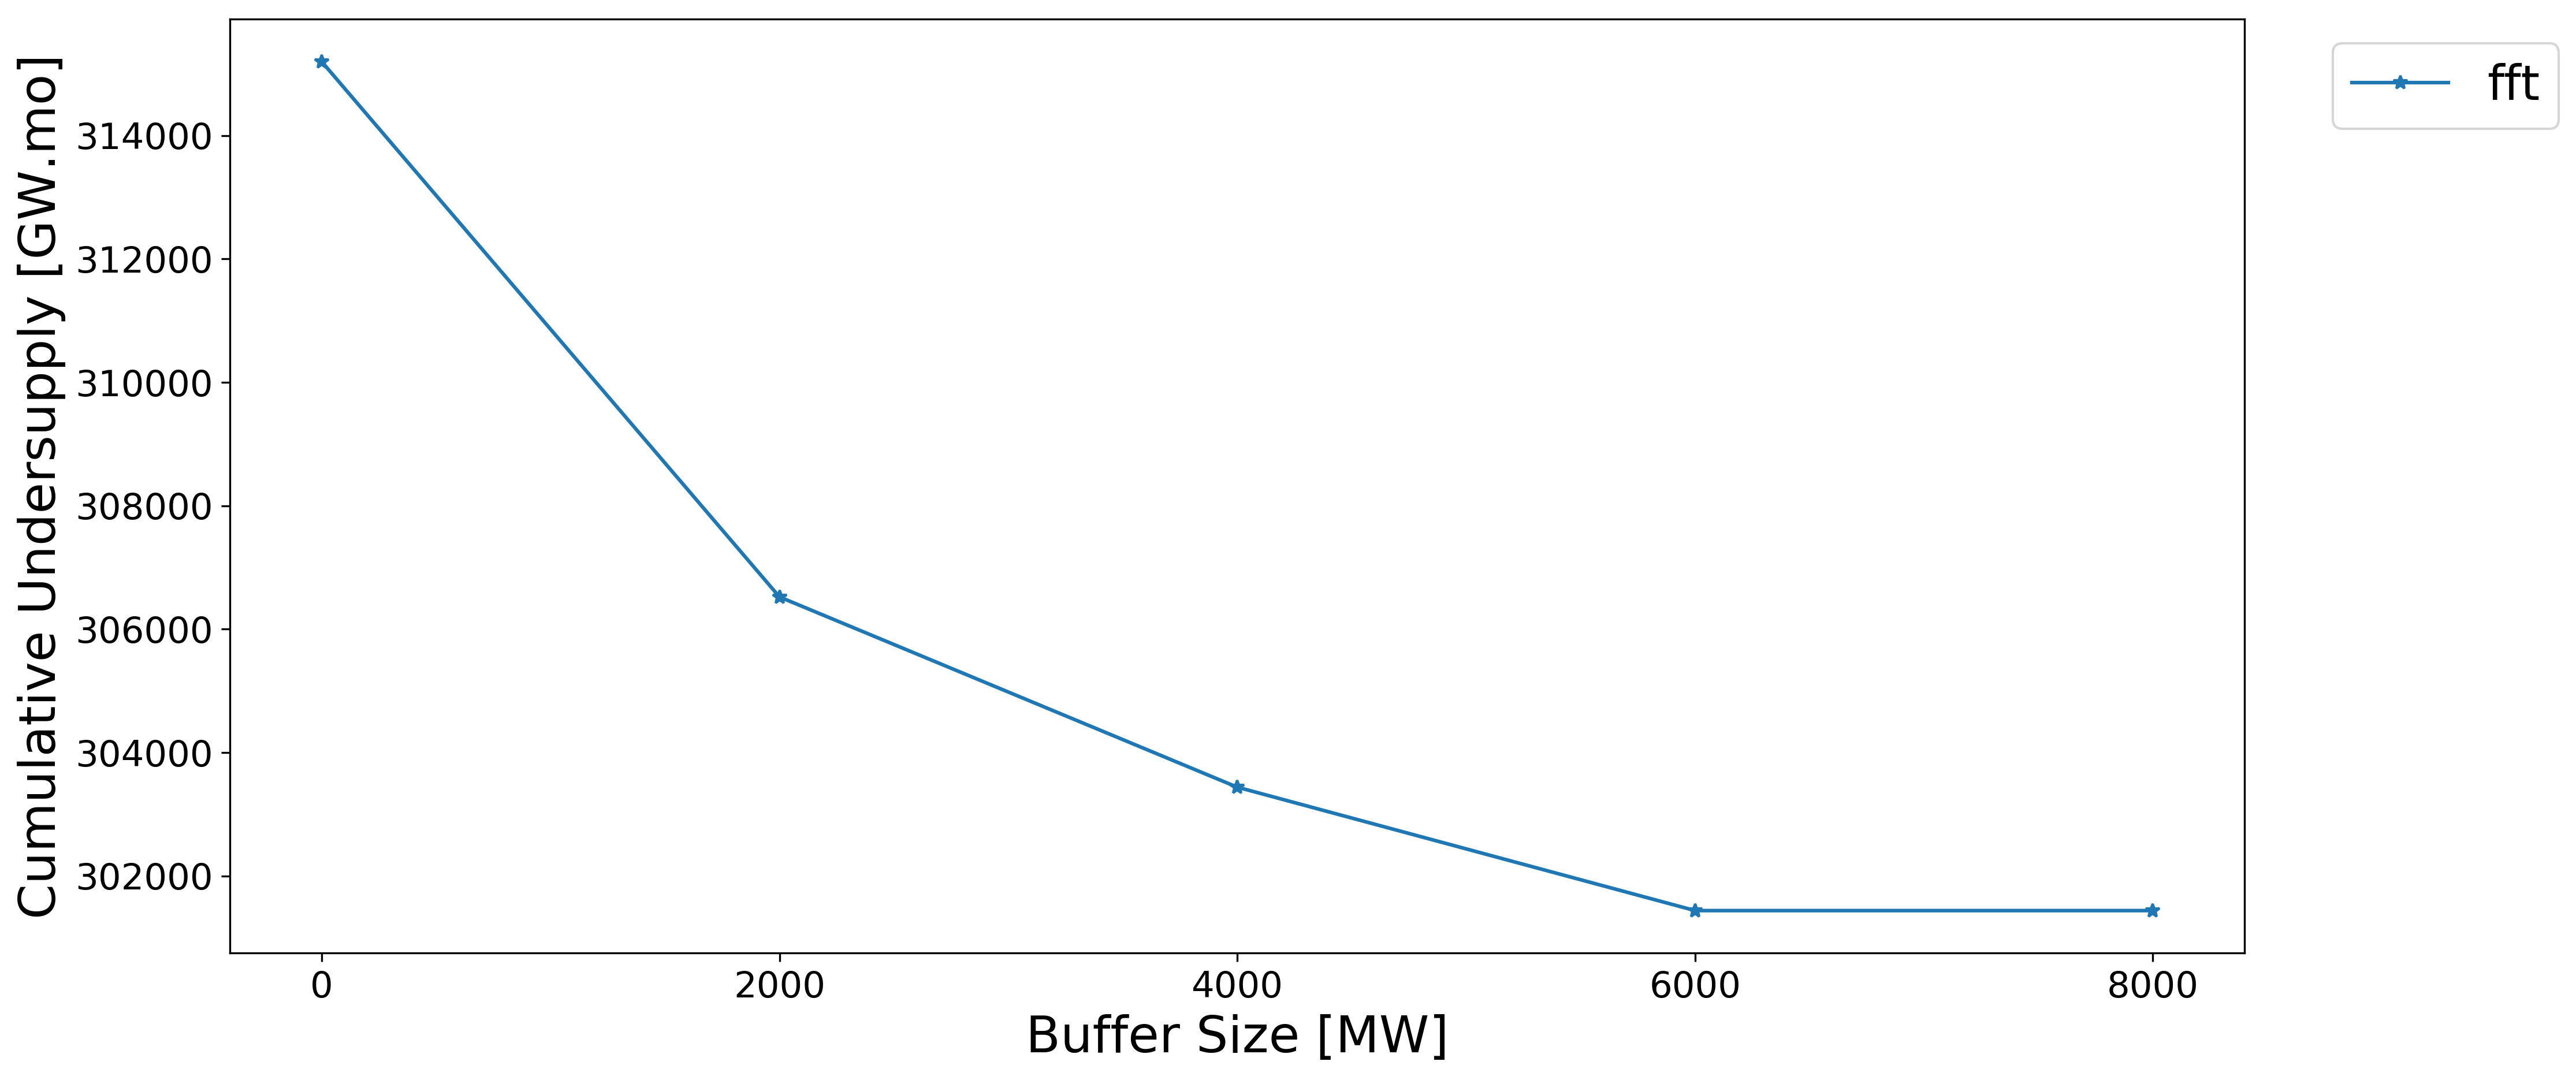
\includegraphics[width=0.8\textwidth]{../paper/figures/24-sens-buffer}
        \end{center}
              \caption{Sensitivity Analysis of Power buffer size on cumulative 
              undersupply of Power for EG01-EG24 transition scenarios 
              with linearly increasing power demand using the fft prediction method.}
      \end{figure}
\end{frame}

\begin{frame}
    \frametitle{Sensitivity Analysis of Power Buffer}
    \textbf{EG01-30}: Linearly Increasing Power Demand
    \begin{figure}[htbp!]
        \begin{center}
          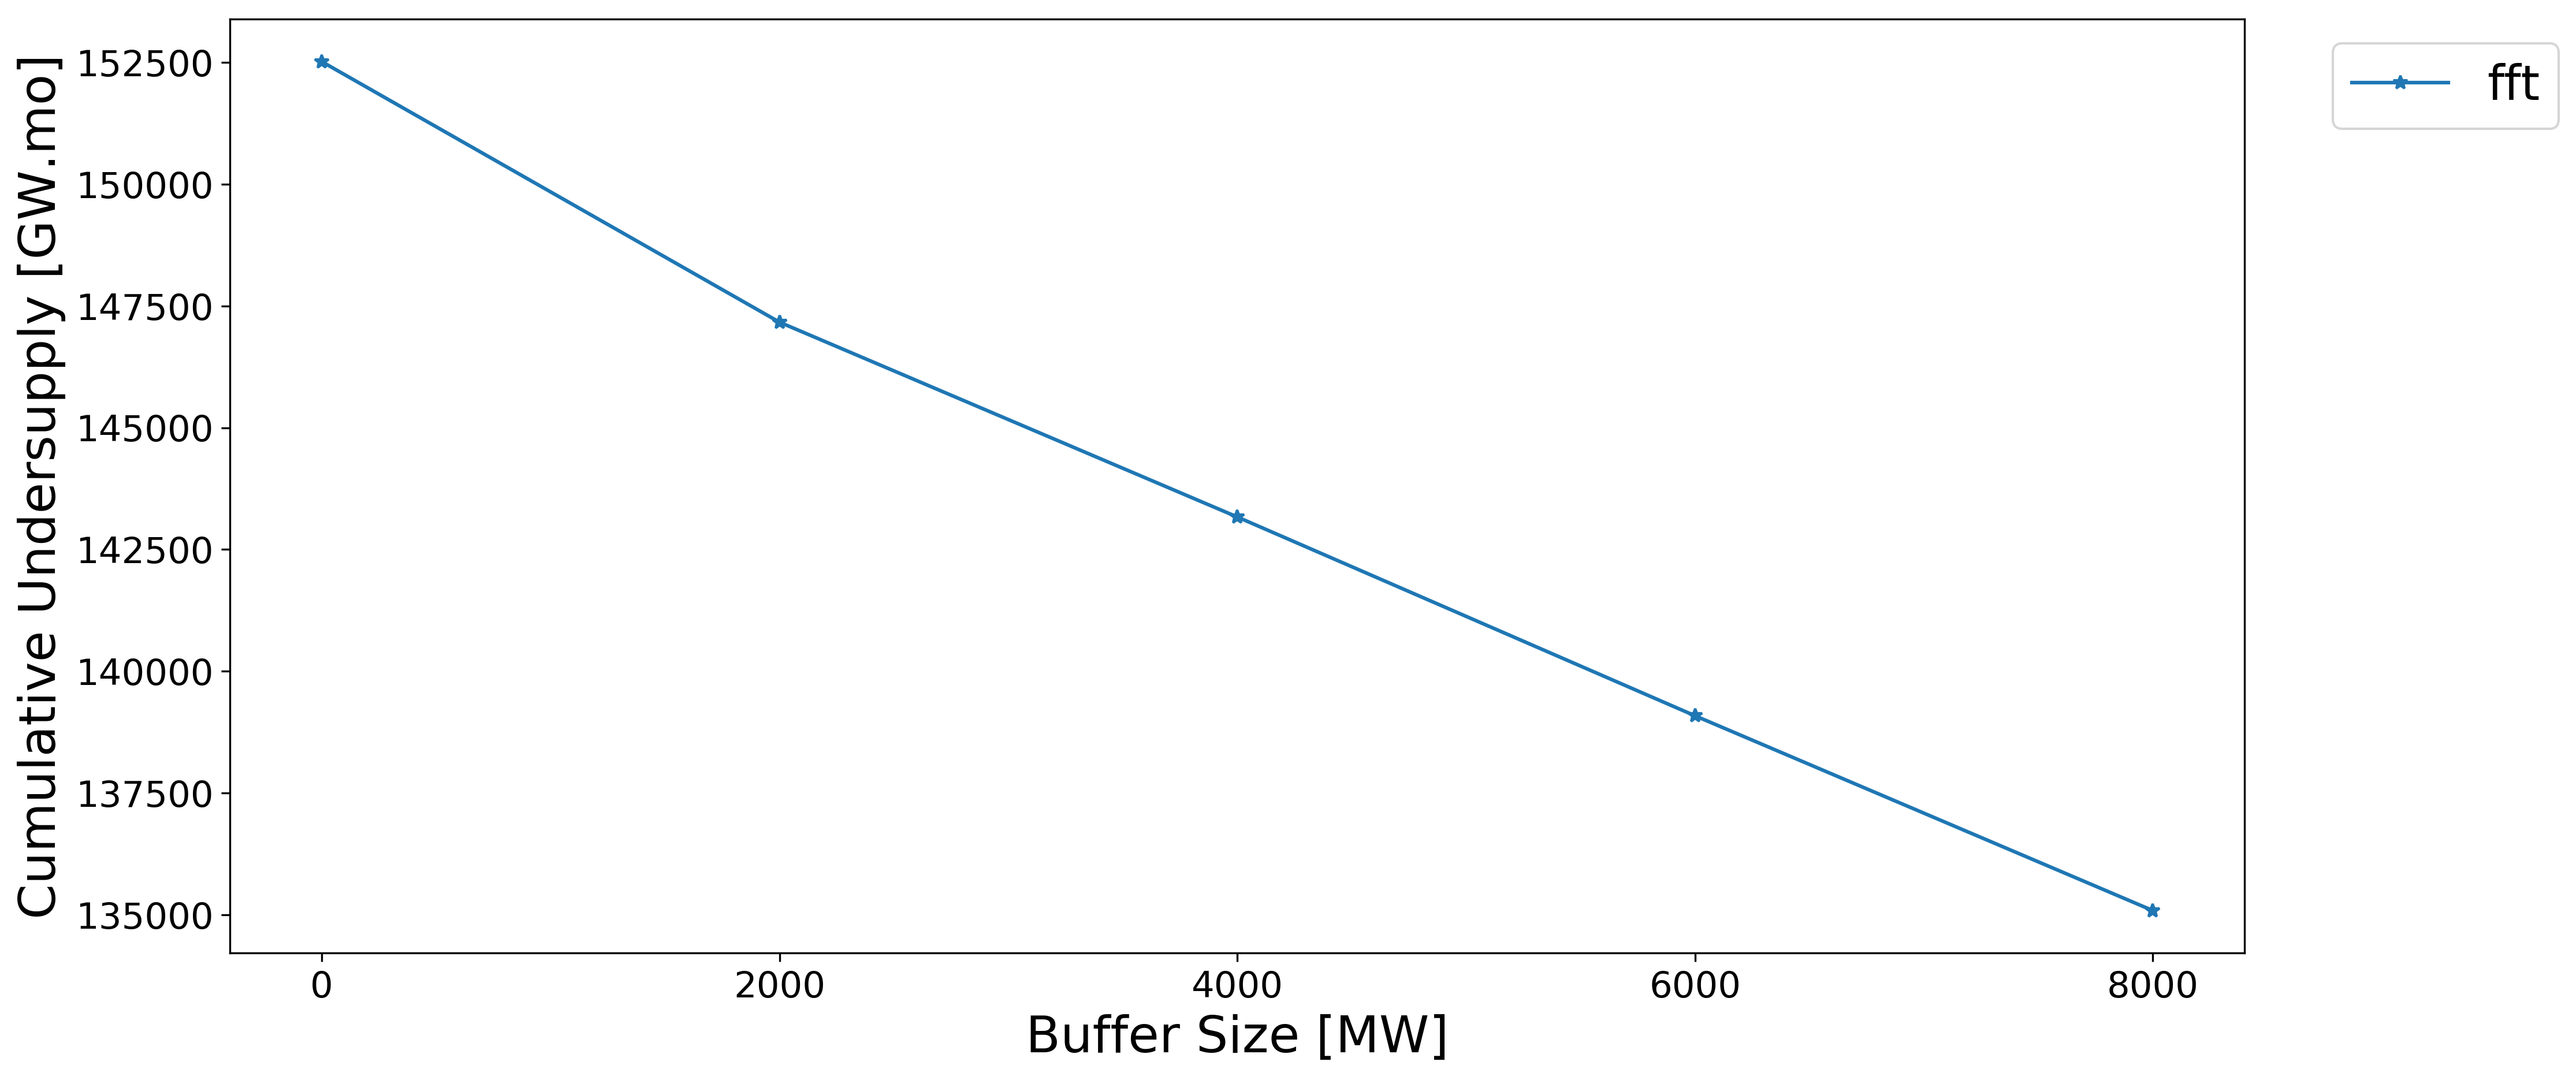
\includegraphics[width=0.8\textwidth]{../paper/figures/30-sens-buffer}
        \end{center}
              \caption{Sensitivity Analysis of Power buffer size on cumulative 
              undersupply of Power for EG01-EG30 transition scenarios 
              with linearly increasing power demand using the fft prediction method.}
      \end{figure}
\end{frame}

\begin{frame}
  \frametitle{Sensitivity Analysis of Power Buffer}
  \textbf{Main Takeaway}
  \\
  The best power supply buffer for each transition scenario is: 
  \begin{enumerate}
    \item EG01-23 Constant Power Demand: 0 MW
    \item EG01-24 Linearly Increasing Power Demand: 6000 MW
    \item EG01-29 Constant Power Demand: 0 MW
    \item EG01-30 Linearly Increasing Power Demand: 8000 MW 
\end{enumerate}
\end{frame}